% -- Ogmg performance results
\section{Performance Results}\label{sec:performanceResults}

In this section we present some serial and parallel performance results.


\noindent Notation:
The normalized CPU time TR10M can be used to compare results from different grids and different numbers of processors.
It is a normalized {\em average time to reduce the residual by a factor of 10}. The average time is normalized 
by dividing by the number of grid points (in millions) and multiplying by the number of processors: 
\begin{eqnarray*}
 \Nc_g &=& \mbox{number of grid points}, \\
 N_p &=& \mbox{number of processors}, \\
 \mbox{TR10} &=& \mbox{average CPU time (s) to reduce the residual by a factor of $10$}, \\
 \mbox{TR10M} &=& \mbox{average CPU time (s) to reduce the residual by a factor of $10$ per million grid points per processor} \\
              &=& N_p \times \mbox{TR10M}/( \Nc_g/10^6) .
\end{eqnarray*}
Values for TR10M for Ogmg should be roughly indepdendent of the number of grid points and number of processors. 
The {\em normalized memory usage} is indicated by the number of {\em reals-per-grid-point} (RPG)
\begin{eqnarray*}
 \mbox{RPG} &=& (\mbox{total memory usage (btyes)})/(\mbox{number-of-grid-points} \times (8~\mbox{bytes/real}))
\end{eqnarray*}

NOTE: The memory usage reported in the tables is the entire memory used by the ogmgt test program. 

% ---------------------------------------------------------------------------------------------------
\clearpage
\subsection{Second-order accurate : comparision between Ogmg and PETSc solvers}

Here are results from solving Poisson's equation to second-order accuracy.

The serial runs were performed on a Intel Xeon 2.3Ghz quad core.

The parallel runs were performed on the Hera Cluster, AMD Opteron cluster, with sixteen 2.3GHz processors/node, 
and 32GB memory per node.


\begin{table}[hbt]
\begin{center}
\begin{tabular}{|c|c|c||c|c|c||c|c|c|} \hline 
      & & & \multicolumn{2}{|c|}{CPU: TR10M} &   & \multicolumn{2}{|c|}{Mem: RPG} &   Memory  \\
   Grid          &  Pts     &  $N_p$   &  Ogmg     &  BICGS(1)  & Speed-up       &   Ogmg   &  PETSc       &  Ratio \\ \hline
 sq2048          & $4.2$M   & serial   &  $.067$   & $7.2$      & $107$          & $7.3$    & $ 63 $       & $8.6$ \\ 
 sq2048          & $4.2$M   &      1   &  $.20$    & $12.5$     & $62.$          & $8.0$    & $ 64 $       & $ 8 $ \\ 
 cic64           & $7.3$M   &      1   &  $.31$    & $23.4$     & $75.$          & $8.7$    & $ 59 $       & $6.7$ \\ 
 tcilc64         & $23.$M   &      8   &  $.53$    & $82.6$     & $156$          & $9.4$    & $ 68 $       & $7.3$ \\ 
\hline % 3D : 
 box256          & $18$M    &     16   &  $.41$    & $14.8$     & $36 $          & $14 $    & $148 $       & $11$ \\ 
 box256          & $18$M    &     32   &  $.56$    & $12 $      & $21 $          & $18 $    & $154 $       & $8.5$ \\ 
% sphere4         & $16$M    &      8   &  $1.1$    & $??  $     & $?? $          & $20 $    & $    $       & $?? $ \\ 
 sphere4         & $16$M    &     16   &  $1.5$    & $242$      & $161$          & $24 $    & $149 $       & $6.2$ \\ 
 sphere4         & $16$M    &     32   &  $2.5$    & $148$      & $59.$          & $31 $    & $159 $       & $5.2$ \\ 
 sphere8         & $125$M   &     64   &  $2.0$    & $556$      & $278$          & $20 $    & $143 $       & $7.2$ \\ 
\hline 
\end{tabular}
\end{center}
\caption{Performance of Ogmg for solving Poisson's equation to fourth-order accuracy on various grids. Comparison is made to 
the Krylov solver PETSC solver bi-CG stab with ILU(1) from PETSc.
TR10M is a normalized CPU time. RPG is the memory usage in reals-per-grid-point.
}
\label{tab:performanceSecondOrder} 
\end{table}

%- \begin{table}[hbt]
%- \begin{center}
%- \begin{tabular}{|c|c|c||c|c|c||c|c|c|} \hline 
%-       & & & \multicolumn{2}{|c|}{CPU: TR10M} &   & \multicolumn{2}{|c|}{Memory/proc Mb} &   Memory  \\
%-    Grid          &  Pts     &  $N_p$   &  Ogmg     &  BICGS(1)  & Speed-up       &   Ogmg            &  PETSc       &  Ratio \\ \hline
%-  square2048      & $4.2$M   & serial   &  $.067$   & $7.2$     & $107$          & $235$             & $2025$       & $8.6$ \\ 
%-  square2048      & $4.2$M   &      1   &  $.20$    & $12.5$     & $62.$          & $255$             & $2040$       & $ 8 $ \\ 
%-  cic64           & $7.3$M   &      1   &  $.31$    & $23.4$     & $75.$          & $487$             & $3280$       & $6.7$ \\ 
%-  tcilc64         & $23.$M   &      8   &  $.53$    & $82.6$     & $156$          & $206$             & $1500$       & $7.3$ \\ 
%- \hline % 3D : 
%-  box256          & $18$M    &     32   &  $.56$    & $12 $      & $21 $          & $78 $             & $662 $       & $8.5$ \\ 
%-  sphere4         & $16$M    &      8   &  $1.1$    & $??  $     & $?? $          & $308$             & $??  $       & $?? $ \\ 
%-  sphere4         & $16$M    &     16   &  $1.5$    & $??  $     & $?? $          & $184$             & $1140$       & $?? $ \\ 
%-  sphere4         & $16$M    &     32   &  $2.5$    & $148 $     & $5.9$          & $117$             & $607 $       & $5.2$ \\ 
%-  sphere8         & $125$M   &     64   &  $2.0$    & $??  $     & $???$          & $300$             & $????$       & $???$ \\ 
%- \hline 
%- \end{tabular}
%- \end{center}
%- \caption{Performance of Ogmg for solving Poisson's equation to fourth-order accuracy on various grids. Comparison is made to 
%- the Krylov solver PETSC solver bi-CG stab with ILU(1) from PETSc.
%- TR10M is a normalized CPU time. 
%- }
%- \label{tab:performanceSecondOrder} 
%- \end{table}

\begin{figure}[hbt]
\begin{center}
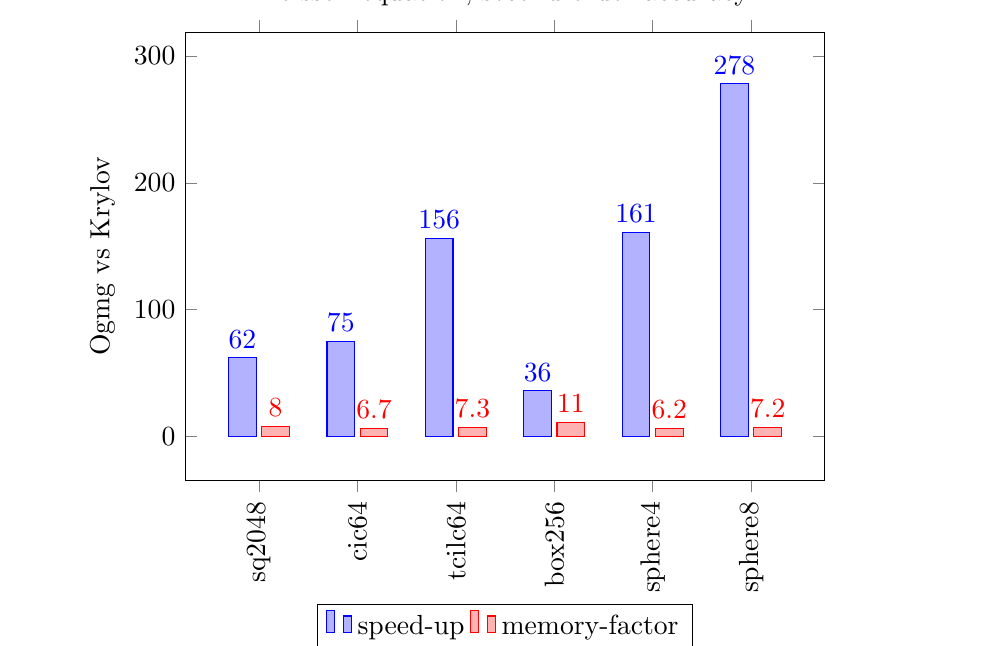
\begin{tikzpicture}
\useasboundingbox (-2,-1.75) rectangle (10,5.75);  % set the bounding box (so we have less surrounding white space)
\begin{axis}[
      ybar,
      x=1.25cm, % distance between entries?
      enlargelimits=0.15,
      legend style={at={(0.5,-0.275)},
          anchor=north,legend columns=-1},
      ylabel={Ogmg vs Krylov},
      symbolic x coords={sq2048,cic64,tcilc64,box256,sphere4,sphere8},
      xtick=data,
      x tick label style= {rotate=90,anchor=east},  % rotate bottom ``tick'' labels
      nodes near coords,
      nodes near coords align={vertical},
      title={Poisson equation, second-order accuracy}
      ]
\addplot coordinates {(sq2048,62) (cic64,75) (tcilc64,156) (box256,36) (sphere4,161) (sphere8,278)};
\addplot coordinates {(sq2048,8) (cic64,6.7) (tcilc64,7.3) (box256,11) (sphere4,6.2) (sphere8,7.2)};
% \addplot coordinates {(tool8,4) (tool9,4) (tool10,4)};
% \addplot coordinates {(tool8,1) (tool9,1) (tool10,1)};
\legend{speed-up,memory-factor}
\end{axis}
% \draw (current bounding box.south west) rectangle (current bounding box.north east);
% \draw[step=1cm,gray] (-2,-2) grid (7,6);
\end{tikzpicture}
\end{center}
\caption{Performance of Ogmg for solving Poisson's equation to {\em second-order accuracy} on various grids.
Ogmg is compared to a Krylov solver (bi-CG stab, ILU(1)) from PETSc.
  The CPU speed-up factor (Ogmg/Krylov) is shown along with the ratio of memory usage (Krylov/Ogmg). For example,
 for the case {\em cic64}, Ogmg is $75$ times faster and uses a factor of $6.7$ times less memory.}
\label{fig:performanceSecondOrder} 
\end{figure}

Note: The serial code results (which is run on tux291) 
may be faster than the parallel code since the default smoother in serial is Red-Black GS which is a better smoother
that the Red-Black Jacobi which is the default smoother in parallel.


Here are the ogen commands used to build the different grids:
\begin{flushleft}
 square2048 : ogen noplot squareArg -order=2 -nx=2048 \\
 cic64 : ogen noplot cicArg -order=2 -interp=e -ml=5 -factor=64 \\
 tcilc64 : ogen -noplot tcilc -order=2 -interp=e -ml=4 -factor=64 \\
 box256    : ogen noplot box -order=2 -nx=256 \\
 sphere4    : ogen -noplot sphereInABox -order=2 -interp=e -factor=4 -ml=4 \\
 sphere8    : ogen -noplot sphereInABox -order=2 -interp=e -factor=8 -ml=5
\end{flushleft}

% ---------------------------------------------------------------------------------------------------
\clearpage
\subsection{Fourth-order accurate : comparision between Ogmg and PETSc solvers}

Here are results from solving Poisson's equation to fourth-order accuracy.

NOTE: RERUN -np=1 with parallel code

% NOTE: results from Overture/ogmg/performance/memo
\begin{table}[hbt]
\begin{center}
\begin{tabular}{|c|c|c||c|c|c||c|c|c|} \hline 
      & & & \multicolumn{2}{|c|}{CPU: TR10M} &   & \multicolumn{2}{|c|}{Mem: RPG} &   Memory  \\
   Grid          &  Pts     &  $N_p$   &  Ogmg     &  BICGS(1)  & Speed-up       &   Ogmg   &  PETSc       &  Ratio \\ \hline
 sq2048          & $4.2$M   &  serial  &  $.12$    & $10.$      & $82.$          & $7.3$    & $112 $       & $15.$ \\ 
 cic64           & $7.3$M   &  serial  &  $.15$    & $13.7$     & $91.$          & $14. $   & $99  $       & $7.3$ \\ 
 tcilc64         & $23.$M   &      8   &  $.93$    & $225$      & $242$          & $10. $   & $133 $       & $13.$ \\ 
\hline % 3D : 
 box256          & $18$M    &     32   &  $.82$    & $62.$      & $75.$          & $22. $   & $536 $       & $25.$ \\ 
 sphere4         & $16$M    &     32   &  $5.5$    & $2010$     & $360$          & $81.$    & $624 $       & $7.7$ \\ 
 sphere8         & $125$M   &     64   &  $4.7$    & $??  $     & $???$          & $53.$    & $????$       & $???$ \\ 
\hline 
\end{tabular}
\end{center}
\caption{Performance of Ogmg for solving Poisson's equation to fourth-order accuracy on various grids. Comparison is made to 
the Krylov solver PETSC solver bi-CG stab with ILU(1) from PETSc.
TR10M is a normalized CPU time. 
}
\label{tab:performanceFourthOrder} 
\end{table}

%- \begin{table}[hbt]
%- \begin{center}
%- \begin{tabular}{|c|c|c||c|c|c||c|c|c|} \hline 
%-       & & & \multicolumn{2}{|c|}{CPU: TR10M} &   & \multicolumn{2}{|c|}{Memory/proc Mb} &   Memory  \\
%-    Grid          &  Pts     &  $N_p$   &  Ogmg     &  BICGS(1)  & Speed-up       &   Ogmg            &  PETSc       &  Ratio \\ \hline
%-  square2048      & $4.2$M   &  serial  &  $.12$    & $10.$      & $82.$          & $235$             & $3600$       & $15.$ \\ 
%-  cic64           & $7.3$M   &  serial  &  $.15$    & $13.7$     & $91.$          & $751$             & $5500$       & $7.3$ \\ 
%-  tcilc64         & $23.$M   &      8   &  $.93$    & $225$      & $242$          & $228$             & $2920$       & $13.$ \\ 
%- \hline % 3D : 
%-  box256          & $18$M    &     32   &  $.82$    & $62.$      & $75.$          & $93$              & $2300$       & $24.$ \\ 
%-  sphere4         & $16$M    &     32   &  $5.5$    & $2010$     & $360$          & $309$             & $2380$       & $7.7$ \\ 
%-  sphere8         & $125$M   &     64   &  $4.7$    & $??  $     & $???$          & $790$             & $????$       & $???$ \\ 
%- \hline 
%- \end{tabular}
%- \end{center}
%- \caption{Performance of Ogmg for solving Poisson's equation to fourth-order accuracy on various grids. Comparison is made to 
%- the Krylov solver PETSC solver bi-CG stab with ILU(1) from PETSc.
%- TR10M is a normalized CPU time. 
%- }
%- \label{tab:performanceFourthOrder} 
%- \end{table}


\begin{figure}[hbt]
\begin{center}
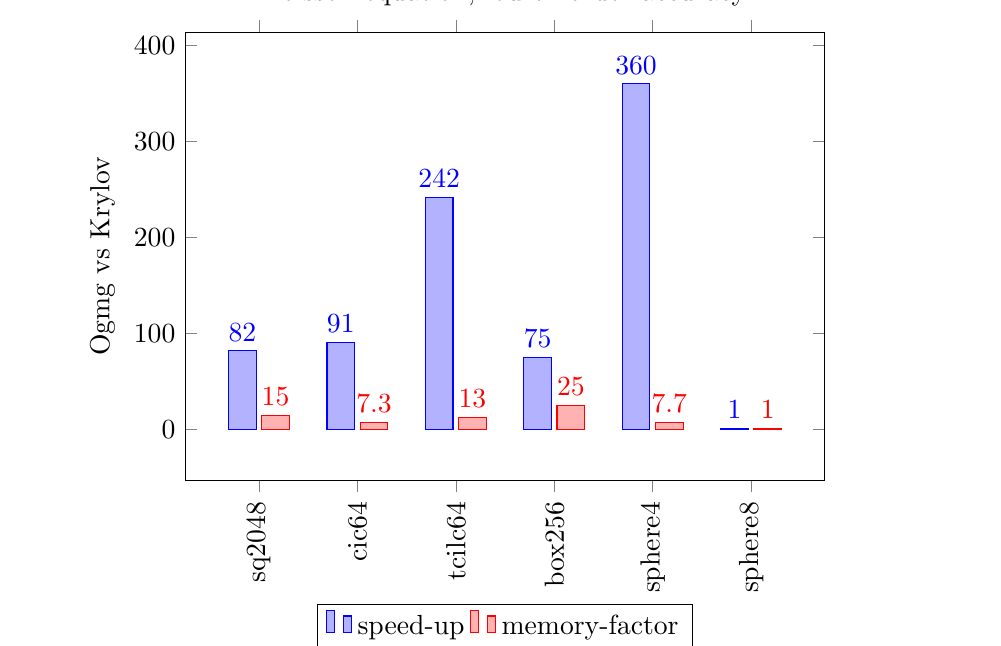
\begin{tikzpicture}
\useasboundingbox (-2,-1.75) rectangle (10,5.75);  % set the bounding box (so we have less surrounding white space)
\begin{axis}[
      ybar,
      x=1.25cm, % distance between entries?
      enlargelimits=0.15,
      legend style={at={(0.5,-0.275)},
          anchor=north,legend columns=-1},
      ylabel={Ogmg vs Krylov},
      symbolic x coords={sq2048,cic64,tcilc64,box256,sphere4,sphere8},
      xtick=data,
      x tick label style= {rotate=90,anchor=east},  % rotate bottom ``tick'' labels
      nodes near coords,
      nodes near coords align={vertical},
      title={Poisson equation, fourth-order accuracy}
      ]
\addplot coordinates {(sq2048,82) (cic64,91) (tcilc64,242)  (box256,75) (sphere4,360) (sphere8,1)};
\addplot coordinates {(sq2048,15) (cic64,7.3) (tcilc64,13)  (box256,25) (sphere4,7.7) (sphere8,1)};
% \addplot coordinates {(tool8,4) (tool9,4) (tool10,4)};
% \addplot coordinates {(tool8,1) (tool9,1) (tool10,1)};
\legend{speed-up,memory-factor}
\end{axis}
% \draw (current bounding box.south west) rectangle (current bounding box.north east);
% \draw[step=1cm,gray] (-2,-2) grid (7,6);
\end{tikzpicture}
\end{center}
\caption{Performance of Ogmg for solving Poisson's equation to {\em fourth-order accuracy} on various grids.
Ogmg is compared to a Krylov solver (bi-CG stab, ILU(1)) from PETSc.
  The CPU speed-up factor (Ogmg/Krylov) is shown along with the ratio of memory usage (Krylov/Ogmg). For example,
 for the case {\em cic64}, Ogmg is $91$ times faster and uses a factor of $7.3$ times less memory.}
\label{fig:performanceFourthOrder} 
\end{figure}

Table~\ref{tab:performanceFourthOrder} and Figure~\ref{fig:performanceFourthOrder} compares Ogmg to a Krylov solver from PETSC. 
The Krylov solver is bi-conjugate gradient stabilized, with ILU(1), reverse Cuthill-McKee ordering, denoted by BICGS(1). 
Ogmg is found to be two-orders of magnitude faster and use an order of magnitude less storage than BICGS(1). 

Note: the case {\em sphere4} in Table~\ref{tab:performanceFourthOrder} was rerun with ILU(3) but the result was only slightly improved,
at the cost of more memory. 



Here are the ogen commands used to build the different grids:
\begin{flushleft}
 square2048 : ogen noplot squareArg -order=4 -nx=2048 \\
 cic64 : ogen noplot cicArg -order=4 -interp=e -ml=5 -factor=64 \\
 tcilc64 : ogen -noplot tcilc -order=4 -interp=e -ml=4 -factor=64 \\
 box256    : ogen noplot box -order=4 -nx=256 \\
 sphere4    : ogen -noplot sphereInABox -order=4 -interp=e -factor=4 -ml=4 \\
 sphere8    : ogen -noplot sphereInABox -order=4 -interp=e -factor=8 -ml=5
\end{flushleft}


%- % Preamble: \pgfplotsset{width=7cm,compat=1.5.1}
%- \begin{tikzpicture}
%- \begin{axis}[
%-       ybar,
%-       enlargelimits=0.15,
%-       legend style={at={(0.5,-0.15)},
%-           anchor=north,legend columns=-1},
%-       ylabel={\#participants},
%-       symbolic x coords={tool8,tool9,tool10},
%-       xtick=data,
%-       nodes near coords,
%-       nodes near coords align={vertical},
%-       ]
%- \addplot coordinates {(tool8,7) (tool9,9) (tool10,4)};
%- \addplot coordinates {(tool8,4) (tool9,4) (tool10,4)};
%- \addplot coordinates {(tool8,1) (tool9,1) (tool10,1)};
%- \legend{used,understood,not understood}
%- \end{axis}
%- \end{tikzpicture}
%- 

%- 
%- 
%- 
%- \begin{table}[hbt]
%- \begin{center}
%- \begin{tabular}{|c|c|c|c|c|c|c|c|} \hline 
%- % \multicolumn{3}{|c|}{} & \multicolumn{3}{|c|}{LFA}  \\ \hline
%- \multicolumn{3}{|c|}{$\omega$-RB-GS} & \multicolumn{3}{|c|}{LFA} & \multicolumn{2}{|c|}{Computed}  \\ \hline
%- % \multicolumn{8}{|c|}{}\multicolumn{3}{|c|}{LFA}\multicolumn{2}{|c|}{Computed}  \\ \hline
%-  $[\nu_1,\nu_2]$ & Galerkin &$\omega$&$\muLoc$ &$\rhoLocTwoGrid$&$\rhoLocThreeGrid$ &$\rho(W)$     &$\rho(V)$\\ \hline\hline
%- %                &          &        &         &                &                   &              &        \\ \hline
%-  $[1,1]$         & No       &   $1$  & $.0625$ & $.074$         & $.104$            & $.061$       & $.092$ \\ 
%-  $[1,1]$         & Yes      &   $1$  & $.0625$ & $.0625$        & $.066$            & $.059$       & $.058$ \\ 
%-  $[1,1]$         & Yes      & $1.10$ & $.0734$ & \fbox{$.0388$} & $.052$            & \fbox{$.034$}& $.037$ \\ \hline 
%-  $[2,1]$         & No       &   $1$  & $.0335$ & $.0523$        & $.074$            & $.044$       & $.064$ \\ 
%-  $[2,1]$         & Yes      &   $1$  & $.0335$ & $.0284$        & $.040$            & $.026$       & $.034$ \\ 
%-  $[2,1]$         & Yes      & $1.10$ & $.0440$ & \fbox{$.0157$} & $.024$            &\fbox{$.014$} & $.015$ \\ 
%- \hline \hline
%- \multicolumn{8}{|c|}{Second-order accuracy, two-dimensional, 5 point Laplacian.}  \\
%- \hline 
%- \end{tabular}
%- \end{center}
%- \caption{Smoothing rates and asymptotic convergence factors for various $\omega$-RB-GS cycles compared to the computed
%- convergence rates for a $1024^2$ square.}
%- \label{tab:ratesSecondOrder2D} 
%- \end{table}